\documentclass{standalone}
\usepackage{ tikz }
\usepackage{ xparse }
\usepackage{../../../macros}
\usepackage{amssymb}

\usetikzlibrary{shapes.gates.logic.US}

\begin{document}
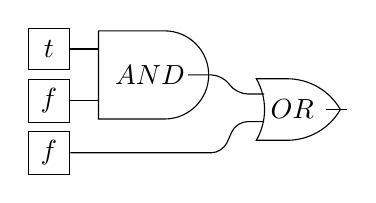
\begin{tikzpicture}[yscale=-1,x=1em,y=1.25em]
        
    \node [draw, anchor=east, minimum width=1.5em, minimum height=1.5em] at (0,0) {$\mf{t}$};
    \node [draw, anchor=east, minimum width=1.5em, minimum height=1.5em] at (0,1.5) {$\mf{f}$};
    \node [draw, anchor=east, minimum width=1.5em, minimum height=1.5em] at (0,3) {$\mf{f}$};
    \draw [rounded corners] (0,0) -- (0.5,0) -- (1,0);
    \draw [rounded corners] (0,1.5) -- (0.5,1.5) -- (1,1.5);
    \node [draw, and gate US, anchor=west, minimum width=2em] at (1,0.75) {$\mf{AND}$};
    \draw [rounded corners](4.25,0.75) -- (5.5,0.75) -- (6, 1.3) -- (7,1.3);
    \draw [rounded corners] (0,3) -- (5.5,3) -- (6,2.1) -- (7,2.1);
    \node [draw, or gate US, anchor=west, minimum width=2em] at (7,1.75) {$\mf{OR}$};
    \draw (9.25,1.75) -- (10,1.75);

\end{tikzpicture}
\end{document}